\documentclass{article}

\usepackage{tikz}
\usepackage{graphicx}
\usepackage{placeins}

\newcommand{\nl}{\\[6pt]}
\newcommand{\dl}{\\[12pt]}

\begin{document}
\title{Abstract argumentation frameworks - overview and illustration}
\author{Patrick Bellositz}
\date{}
\maketitle

\section{Introduction}

\section{Definitions}
\textbf{Definition 1} An \emph{argumentation framework} $F$ is a pair $(A,R)$, where $A$ is a set of arguments and $R$ is a set of attack relations.\dl
\textbf{Definition 2} \emph{Attack relations} $R\subseteq A\times A$ represent attacks. The pair $(a,b)$, where $a,b\in A$ means $a$ \emph{attacks} $b$.\dl
\textbf{Example 1} Imagine we have 3 arguments $a_1$, $a_2$, and $b$.\nl
			\begin{tabular}{p{0.5cm}p{0.5cm}l}
			& $a_1$ & = ''Blue is the most beautiful of all colors.''\\
			& $b$ & = ''No, black is much more beautiful!''\\
			& $a_2$ & = ''That's wrong, black isn't even a color.''
			\end{tabular}\nl
These arguments obviously contain 2 attacks. Argument $b$ attacks argument $a_1$ and in turn argument $a_2$ attacks argument $b$.\nl
This results in the framework $F=(A,R)$, where $A=\{a_1,a_2,b\}$ and $R=\{(b,a_1),(a_2,b)\}$.\dl
As writing an argument framework in sets might become hard to read with increasing set sizes, it is also possible to write every framework as a graph $(V,E)$, where $V=A$ and $E=R$. The graph in our example looks like this:\dl

\FloatBarrier
	\begin{figure}[h]
		\centering
		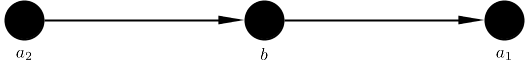
\includegraphics[width=\linewidth]{graphs/ex1.png} %causes underfull hbox and Remark 1 isn't in line with the other txtbf's
		\caption{Example graph 1}
	\end{figure}
\FloatBarrier

\textbf{Remark 1} Let $S$ be a set of arguments. If $a\in S$ and there is an attack $(a,b)\in R$ we say $S$ \emph{attacks} $b$.\dl
\textbf{Definition 3} Let $S$ be a set of arguments. It is \emph{conflict-free}, if $\forall a \forall b\ a,b\in S, (a,b)\notin R$.\dl
\textbf{Example 2} (Continuation of Example 1) As no argument attacks itself, $\{a_1\}$, $\{a_2\}$ and $\{b\}$ each are conflict-free. $\{a_1,a_2\}$ is also a conflict-free set, since there exists no attack relation containing $a_1$ and $a_2$. The empty set is always conflict-free.\\
Since there is an attack relation between $b$ and each of the other arguments, there are no other conflict-free sets.\nl
Thus the set of conflict-free sets is $cf(F)=\{\emptyset,\{a_1\},\{a_2\},\{b\},\{a_1,a_2\}\}$.\dl
\textbf{Definition 4} An argument $a$ is \emph{defended} by a set $S$, if for every attack $(b,a)\in R$ there is an attack $(c,b)$, where $c\in S$. If this is the case $S$ \emph{defends} $a$.\dl
\textbf{Definition 5} Let $S$ be a conflict-free set. It is called an \emph{admissible extension} if it defends each $a\in S$.\dl
\textbf{Example 3} (Continuation of Example 2) Of the conflict-free sets only $\{a_2\}$ and \(\emptyset\) don't get attacked. They are admissible. $\{a_1,a_2\}$ gets attacked via the attack relation $(b,a_1)$, but $a_1$ gets defended through $(a_2,b)$, making it also admissible.\\
$\{b\}$ and $\{a_1\}$ are not admissible since they don't defend their arguments.\nl
Thus the set of admissible extensions is $adm(F)=\{\emptyset,\{a_1,a_2\},\{a_2\}\}$.\dl
\textbf{Definition 6} Let $S$ be an admissible extension. It is called a \emph{preferred extension} if for each $S'\subseteq A$, that is an admissible extension, $S\not\subset S'$.\dl
\textbf{Example 4} (Continuation of Example 3) $\emptyset\subset\{a_2\}$, therefore \(\emptyset\) is not a preferred extension. $\{a_2\}\subset\{a_1,a_2\}$, therefore $\{a_2\}$ is not a preferred extension.\\
Since all other admissible extensions are proper subsets of $\{a_1,a_2\}$, it is a preferred extension.\nl
Thus the set of preferred extensions is $prf(F)=\{\{a_1,a_2\}\}$.\dl
\textbf{Definition 7} Let $S$ be a conflict-free set. It is called a \emph{stable extension} if for each $a\not\in S$ there is exists an attack $(b,a)\in R$ where $b\in S$.\dl
\textbf{Example 5} (Continuation of Example 2) \dl %is it, was the definition really of conflict-free sets, not admissible ones?
\textbf{Definition 8} Let $S$ be an admissible extension. It is called a \emph{complete extension} if for each $a\not\in S$, $S\cup \{a\}$ is not an admissible extension.\dl
\textbf{Example 6} (Continuation of Example 3) \dl %todo
\textbf{Definition 9} The (unique) \emph{grounded extension} is defined by $\bigcap\limits_{i=1}^n{S_i}$, where $\{S_1,...,S_n\}$ is the set of all complete extensions.\dl
\textbf{Example 7} (Continuation of Example 6) \dl %todo

\section{Observations}

\FloatBarrier
	\begin{figure}[!htb]
		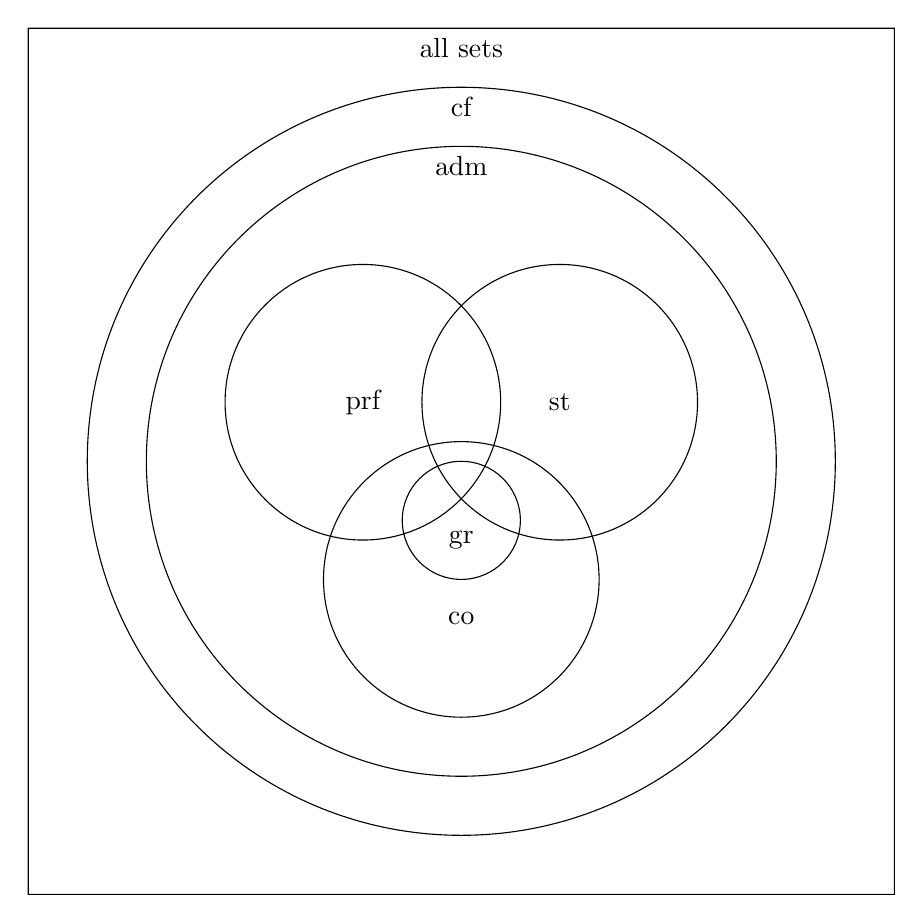
\begin{tikzpicture}[fill=white]
			\scope
				\clip (-2,-2) rectangle (2,2)
					(1,0) circle (1);
				\fill (0,0) circle (1);
			\endscope
			\scope
				\clip (-2,-2) rectangle (2,2)
					(0,0) circle (1);
				\fill (1,0) circle (1);
			\endscope
			\draw (3.5,3.5) circle (4.75) (3.5,7.75) node [text=black,above] {cf}
				(3.5,3.5) circle (4) (3.5,7) node [text=black,above] {adm}
				(2.25,4.25) circle (1.75) node [text=black] {prf}	
				(4.75,4.25) circle (1.75) node [text=black] {st}
				(3.5,2) circle (1.75) (3.5, 1.5) node [text=black] {co}
				(3.5,2.75) circle (.75) (3.5, 2.5) node [text=black] {gr}
				(-2,-2) rectangle (9,9) (3.5,8.75) node [text=black]{all sets};
		\end{tikzpicture}
		\caption{Relation between extension types}
	\end{figure}
\FloatBarrier

\section{Application}
\subsection{Introduction}
In this section the usage and implementation details of the aforementioned program illustrating the computation of the different extension types is provided.

\subsection{Creation of a framework}
On starting the application the user is presented with an input mask. It consists of ten rows, each representing an argument and a button labeled "show graph".

\FloatBarrier
	\begin{figure}[!htb]
		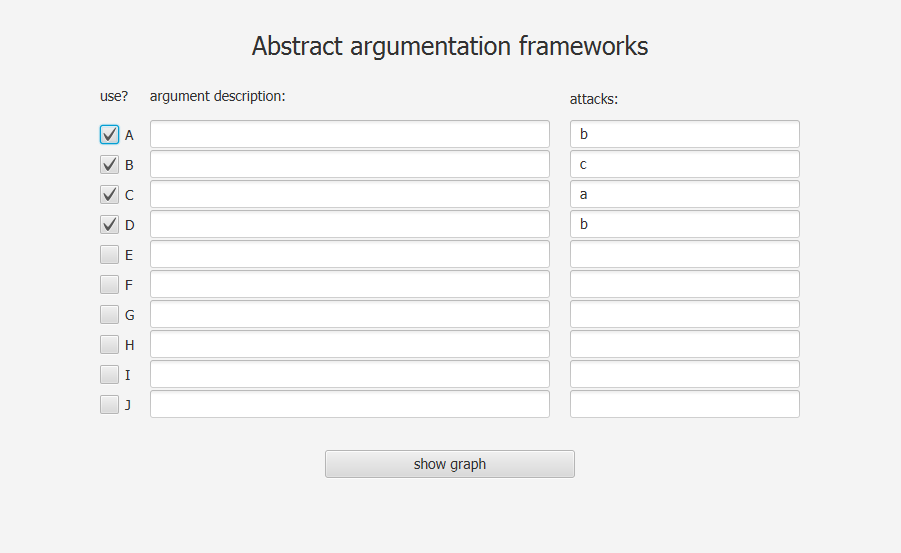
\includegraphics[width=\linewidth]{pics/input.png}
		\caption{Input mask}
	\end{figure}
\FloatBarrier

\subsection{Argumentation graph}
Once a framework is created and "show graph" was clicked a graphical representation of it is shown alongside buttons to compute extensions and an area dedicated to showing computation results.

\FloatBarrier
	\begin{figure}[!htb]
		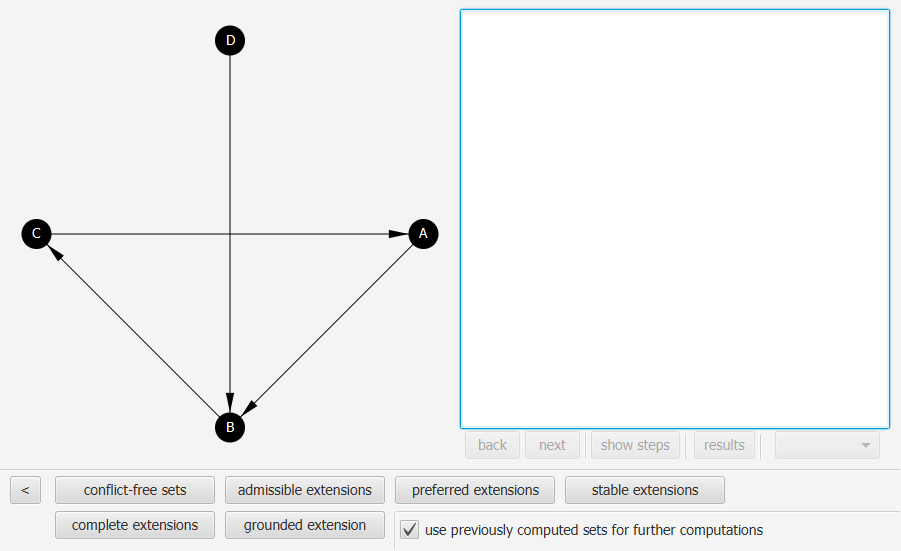
\includegraphics[width=\linewidth]{pics/demo.png}
		\caption{Demonstration view}
	\end{figure}
\FloatBarrier

\subsection{stuff comes here}

\end{document}